\documentclass[12pt,letterpaper]{article}

% --- PAQUETES TIPOGRÁFICOS Y BÁSICOS ---
\usepackage[utf8]{inputenc}
\usepackage[spanish]{babel}
\usepackage{microtype}            % Mejora la justificación
\usepackage{newtxtext,newtxmath}  % Tipografía elegante compatible con pdfLaTeX
\usepackage{graphicx}
\usepackage{amsmath}
\usepackage{geometry}
\usepackage{hyperref}
\usepackage{caption}
\usepackage{enumitem}
\usepackage{fancyhdr}
\usepackage{titlesec}
\usepackage{xcolor}
\usepackage{float}     % para usar [H]
\usepackage{placeins}  % para \FloatBarrier
\usepackage{datetime2}
\usepackage{listings}
\usepackage{minted}

\setminted{
    breaklines=true,
    breakanywhere=true,
    fontsize=\small,
    frame=single,
    linenos
}

% --- GEOMETRÍA DE PÁGINA ---
\geometry{
  letterpaper,
  margin=1in,
  headheight=15pt % Corrige warning de fancyhdr
}

% --- PÁRRAFOS Y LÍNEA ---
\setlength{\parindent}{1.5em}   % Sangría inicial en párrafos
\setlength{\parskip}{0.4em}     % Pequeño espacio entre párrafos
\linespread{1.05}               % Ligeramente más aire entre líneas
\raggedbottom                   % Evita estiramientos verticales feos

% --- LISTAS COMPACTAS (sin perder legibilidad) ---
\setlist[itemize]{topsep=4pt,itemsep=2pt,parsep=2pt}
\setlist[enumerate]{topsep=4pt,itemsep=2pt,parsep=2pt}

% --- CAPTIONS ---
\captionsetup[figure]{labelfont=bf,font=small}
% \captionsetup[table]{labelfont=bf,font=small}
% \captionsetup[listing]{labelfont=bf,font=small,name=Listado}

% --- HYPERREF ---
\hypersetup{
  colorlinks=true,
  linkcolor=blue!50!black,
  urlcolor=teal!60!black,
  citecolor=purple!60!black,
  pdftitle={SimpleImgProcessing},
  pdfpagemode=UseOutlines
}

% --- ENCABEZADOS Y PIES ---
\pagestyle{fancy}
\fancyhf{}
\fancyhead[L]{Actividad 2.2 Google Colab: SimpleImg\_Processing - Equipo 5}
\fancyhead[R]{\thepage}
\renewcommand{\headrulewidth}{0.4pt}
\renewcommand{\footrulewidth}{0pt}
\setlength{\headheight}{15pt} % Corrige el warning de fancyhdr

% --- ESTILO DE SECCIONES ---
\titleformat{\section}{\large\bfseries}{\thesection}{0.6em}{}
\titleformat{\subsection}{\normalsize\bfseries}{\thesubsection}{0.6em}{}
\titleformat{\subsubsection}{\normalsize\itshape}{\thesubsubsection}{0.6em}{}
\titlespacing*{\section}{0pt}{0.8em}{0.4em}
\titlespacing*{\subsection}{0pt}{0.6em}{0.3em}
\titlespacing*{\subsubsection}{0pt}{0.5em}{0.25em}

% --- RUTA DE IMÁGENES (opcional) ---
% \graphicspath{{figuras/}}

% --- MODO DRAFT PARA COMPILACIÓN RÁPIDA ---
% Si tienes problemas de timeout, descomenta la siguiente línea:
% \usepackage[draft]{graphicx}  % Esto evita cargar las imágenes completas

% ==============================
% INICIO DEL DOCUMENTO
% ==============================
\begin{document}

% ========== CARÁTULA ==========
\begin{titlepage}
  \centering
  \vspace*{0.5cm}
  
\includegraphics[width=0.5\textwidth]{logo.jpg}\par
  \vspace{1.2cm}

  {\Large\scshape Instituto Tecnológico y de Estudios Superiores de Monterrey\par}
  \vspace{2.2cm}

  {\huge\bfseries Actividad 2.2 Google Colab\par
   \vspace{0.2cm}
   \emph{SimpleImg\_Processing}\par}
  \vspace{2.2cm}

  \begin{center}
    {\Large\bfseries Equipo 5\par}
    \vspace{1em}
    \begin{tabular}{r l}
      \textbf{A01796323} & Benjamín Cisneros Barraza \\
      \textbf{A01066264} & Carlos Pano Hernandez \\
      \textbf{A01795590} & Edgar Omar Cruz Mendoza \\
      \textbf{A01275322} & Jonatan Israel Meza Mendoza \\
    \end{tabular}
  \end{center}
  
  \vspace{1.2cm}

  \begin{flushleft}
    \normalsize \textbf{Profesor Titular:} Dr. Gilberto Ochoa Ruiz\\
    \normalsize \textbf{Profesor Asistente:} MIP Ma. del Refugio Meléndez Alfaro\\
    \normalsize \textbf{Profesor Tutor:} Iván Reyes Amezcua
  \end{flushleft}

  \vfill

  \begin{flushright}
    \normalsize Visión computacional para imágenes y video\\
    \normalsize 21 de Septiembre de 2025
  \end{flushright}
\end{titlepage}

\setcounter{page}{1} % Reinicia numeración tras la carátula

% ========== RESUMEN ==========
\section*{Resumen}

Este proyecto presenta una exploración práctica de técnicas fundamentales de procesamiento de imágenes a nivel de píxel, aplicadas mediante Python y OpenCV. Se implementaron y analizaron transformaciones como la \textbf{transformación logarítmica}, el \textbf{estiramiento de contraste}, la \textbf{ecualización del histograma}, la \textbf{inversión negativa}, la \textbf{corrección de gamma} y la \textbf{sustracción de imágenes}. Cada técnica fue evaluada visualmente y mediante histogramas para demostrar su impacto en la mejora del contraste, la revelación de detalles ocultos y la detección de cambios en imágenes. Los resultados muestran cómo estas herramientas pueden ser aplicadas en contextos reales como la detección de billetes falsos, el análisis médico y la vigilancia de seguridad, destacando su utilidad en sistemas de visión computacional.
% ========== OBJETIVOS ==========
\section*{Objetivos}

El objetivo principal de esta actividad es aplicar de forma práctica las técnicas de mejoramiento de imágenes estudiadas previamente en clase, utilizando el entorno colaborativo de Google Colab y la biblioteca OpenCV. A través de la implementación de transformaciones fotométricas pixel a pixel, se busca comprender su impacto en la calidad visual de las imágenes y su utilidad en el contexto de la inteligencia artificial.

Los objetivos específicos son:

\begin{enumerate}
    \item Investigar e implementar tres transformaciones fotométricas pixel a pixel sobre imágenes propias, con el fin de aumentar la diversidad de datos para entrenamiento de modelos de inteligencia artificial.
    \item Aplicar la técnica de inversión de imagen (negativo) en un caso de uso real, justificando su relevancia y mostrando una demostración funcional.
    \item Investigar y aplicar la corrección de gamma en imágenes, explicando su utilidad en contextos específicos como astronomía o imágenes médicas, y presentar una demostración.
    \item Implementar la técnica de sustracción de imágenes para detectar cambios entre dos fotogramas, justificando su aplicación en sistemas de vigilancia o monitoreo.
    \item Documentar el proceso mediante un archivo PDF con capturas de pantalla, resultados y discusión técnica, complementado con un archivo comprimido que contenga el código ejecutable.
\end{enumerate}

\newpage

% ========== TABLA DE CONTENIDOS ==========
\tableofcontents
\newpage

% ========== TABLA DE FIGURAS ==========
\listoffigures
\newpage

% ========== INTRODUCCIÓN ==========
\section{Introducción}

En el campo de la visión por computadora y el procesamiento de imágenes, las transformaciones a nivel de píxel son técnicas fundamentales. Estas transformaciones se utilizan para modificar la intensidad, el \textbf{color o el contraste de una imagen}, lo cual es crucial para tareas como la aumentación de datos en aprendizaje automático, la mejora de imágenes para aplicaciones específicas (p. ej., imágenes médicas, astronomía) y la extracción de características para el análisis. Este proyecto explora varias transformaciones clave a nivel de píxel, incluyendo ajustes fotométricos, la inversión negativa, la corrección de gamma y la sustracción de imágenes.


\newpage

\section{Desarrollo de actividades}

En esta sección se documenta el proceso práctico realizado para aplicar diversas técnicas de procesamiento de imágenes a nivel de píxel, utilizando el entorno colaborativo de Google Colab y la biblioteca OpenCV en Python. Las actividades se enfocan en transformar imágenes propias mediante métodos fotométricos que permiten modificar la intensidad, el contraste y la distribución de los valores de los píxeles. Estas transformaciones son fundamentales en el contexto de la visión computacional, ya que no solo mejoran la calidad visual de las imágenes, sino que también contribuyen a la aumentación de datos, una práctica esencial para entrenar modelos de inteligencia artificial con mayor robustez y precisión.

Cada subsección presenta una técnica específica, su implementación en código, los resultados obtenidos y una justificación basada en literatura especializada. El análisis incluye comparativas visuales y de histogramas que permiten evaluar el impacto de cada transformación sobre las imágenes originales.



\subsection{Transformaciones Pixel a Pixel}

Las transformaciones pixel a pixel son técnicas fundamentales en el procesamiento de imágenes, especialmente útiles en la aumentación de datos para entrenar modelos de inteligencia artificial. En este proyecto se aplicaron tres transformaciones fotométricas sobre imágenes propias: transformación logarítmica, estiramiento de contraste y ecualización del histograma. A continuación se describe cada una con su respectiva implementación, análisis y justificación.

Como primer paso en el desarrollo de las actividades, se realizó la carga de tres imágenes propias desde el carrete personal de los integrantes del equipo. Estas imágenes fueron seleccionadas por su diversidad en contenido y condiciones de iluminación, con el objetivo de evaluar el comportamiento de las transformaciones fotométricas aplicadas posteriormente.

La carga se realizó utilizando la biblioteca \texttt{matplotlib} para su visualización y \texttt{OpenCV} para su procesamiento. A continuación se muestra el código utilizado para desplegar las imágenes en una cuadrícula horizontal:

\begin{minted}{python}
img1 = mpimg.imread('data/img1.jpg')
img2 = mpimg.imread('data/img2.jpg')
img3 = mpimg.imread('data/img3.jpg')
fig, axes = plt.subplots(1, 3, figsize=(15, 5))

axes[0].imshow(img1)
axes[0].set_title('Image 1')
axes[0].axis('off')

axes[1].imshow(img2)
axes[1].set_title('Image 2')
axes[1].axis('off')

axes[2].imshow(img3)
axes[2].set_title('Image 3')
axes[2].axis('off')

plt.tight_layout()
plt.show()
\end{minted}

\begin{figure}[H]
    \centering
    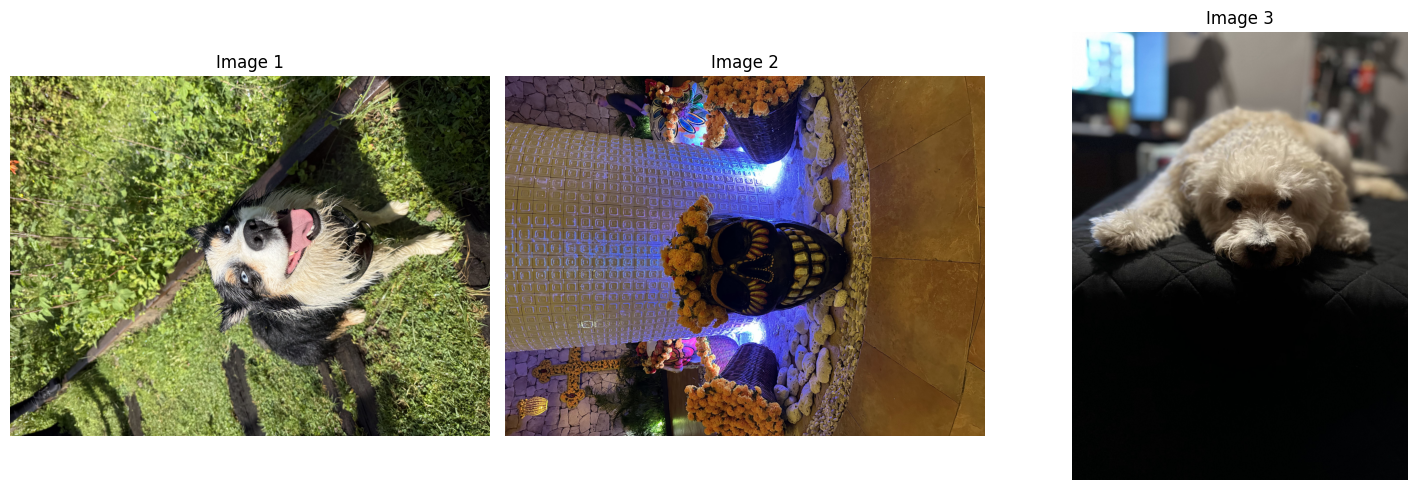
\includegraphics[width=0.9\linewidth]{figuras/carga_imagenes.png}
    \caption{Carga y visualización de imágenes seleccionadas para el proyecto}
    \label{fig:carga_imagenes}
\end{figure}

Estas imágenes (Figura \ref{fig:carga_imagenes}) servirán como base para aplicar las distintas transformaciones pixel a pixel descritas en las siguientes secciones. La diversidad en sus características permitirá observar con mayor claridad los efectos de cada técnica de procesamiento.

\subsubsection{Transformación logarítmica}

La transformación logarítmica es una técnica fotométrica de procesamiento pixel a pixel que permite expandir el rango dinámico de los píxeles oscuros en una imagen, mientras comprime el de los píxeles brillantes. Esta propiedad la hace especialmente útil para revelar detalles en regiones de sombra o baja iluminación, donde la información visual suele estar oculta.

\textbf{Justificación:} Esta transformación es ampliamente utilizada en tareas de aumentación de datos para modelos de inteligencia artificial, ya que permite generar versiones alternativas de una imagen que conservan su estructura pero resaltan detalles que podrían ser ignorados por modelos de aprendizaje profundo. En particular, es útil en dominios como imágenes médicas, astronomía o inspección industrial, donde los detalles en zonas oscuras pueden ser críticos para la toma de decisiones automatizada.

En este proyecto, se aplicó esta transformación a imágenes propias convertidas previamente a escala de grises. El código implementado utiliza la función \texttt{np.log1p()} para aplicar el logaritmo natural a cada valor de intensidad, escalado por una constante que normaliza el resultado al rango de 0 a 255.

\begin{minted}{python}
# Ensure img1 is uint8 RGB for OpenCV ops
if img1.dtype != np.uint8:
    img1_u8 = (cv2.normalize(img1, None, 0, 255, cv2.NORM_MINMAX)).astype(np.uint8)
else:
    img1_u8 = img1

# Convert to grayscale for histogram-based ops
img1_gray = cv2.cvtColor(img1_u8, cv2.COLOR_RGB2GRAY)

# 1) Logarithmic transform (on grayscale)
c_log = 255.0 / np.log1p(255.0)
img_log = (c_log * np.log1p(img1_gray.astype(np.float32))).clip(0, 255).astype(np.uint8)
\end{minted}

\begin{figure}[H]
  \centering
  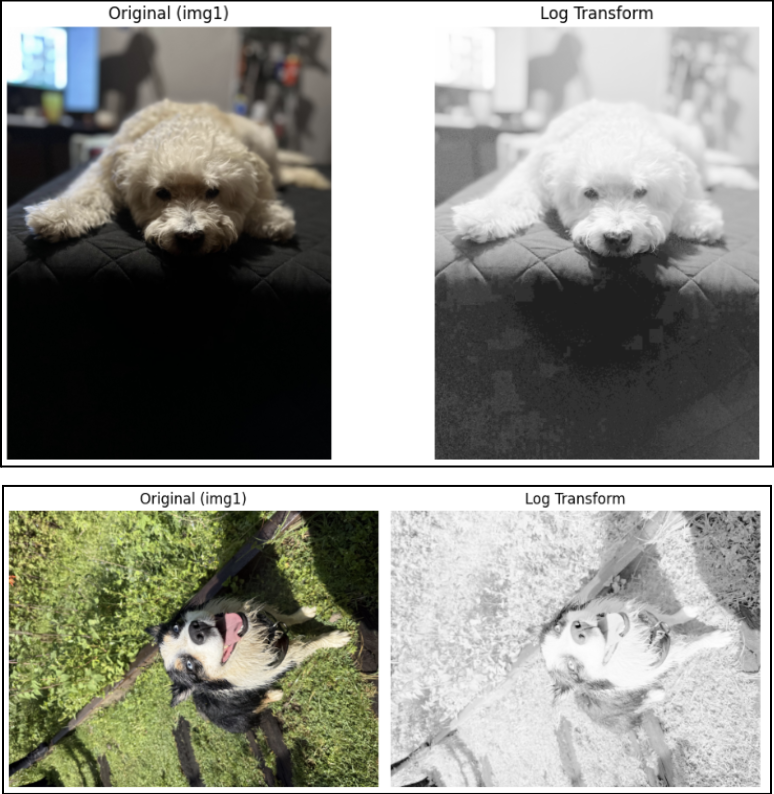
\includegraphics[width=0.5\linewidth]{figuras/transformacion_log.png}
  \caption{Aplicación de transformación logarítmica sobre imagen en escala de grises}
  \label{fig:transformacion_logaritmica}
\end{figure}

\begin{figure}[H]
  \centering
  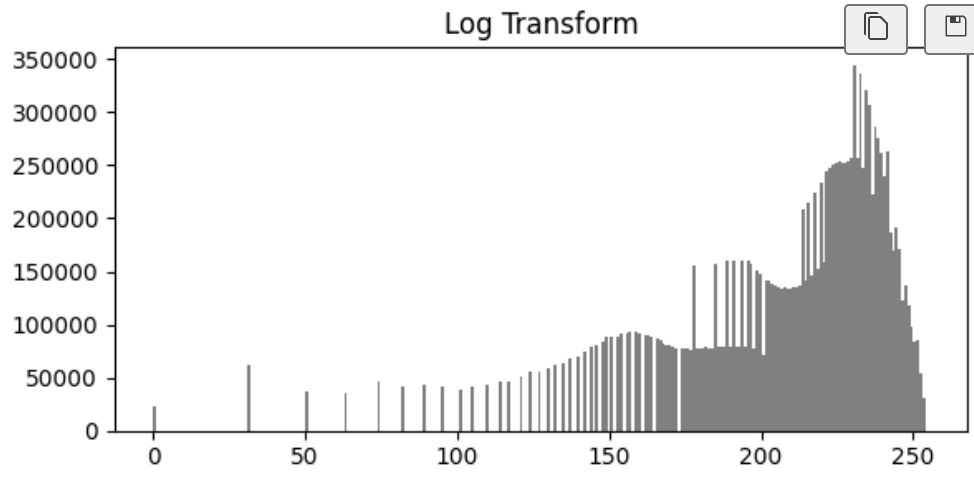
\includegraphics[width=0.5\linewidth]{figuras/histograma_transformacion_logaritmica.png}
  \caption{Transformación Logarítmica: Histograma}
  \label{fig:histograma_transformacion_logaritmica}
\end{figure}


\textbf{Comparativa:} Al aplicar la transformación logarítmica, el histograma de la imagen (Figura~\ref{fig:histograma_transformacion_logaritmica}) se modifica significativamente. Los valores de intensidad originalmente agrupados en el rango bajo se redistribuyen hacia el centro del histograma, lo que indica una mejora en la visibilidad de las zonas oscuras. Esta expansión del rango dinámico en las sombras permite que los detalles ocultos sean más accesibles para algoritmos de detección y clasificación. Como se observa en la Figura~\ref{fig:transformacion_logaritmica}, la transformación permite revelar detalles en zonas oscuras que no eran visibles en la imagen original.

\subsubsection{Estiramiento de contraste}
El estiramiento de contraste es una técnica fotométrica de transformación pixel a pixel que mejora la visibilidad de los detalles en imágenes con bajo contraste. Esta técnica consiste en mapear linealmente el rango de intensidades de píxeles original a un nuevo rango más amplio, típicamente de 0 a 255, lo que permite una mejor distribución de los niveles de gris y una imagen visualmente más clara.

\textbf{Justificación:} Esta transformación es especialmente útil en el contexto de la inteligencia artificial, ya que permite aumentar la diversidad de imágenes de entrenamiento mediante aumentación de datos. Al mejorar el contraste, se facilita la extracción de características relevantes por parte de modelos de aprendizaje profundo, como redes neuronales convolucionales (CNN), lo cual puede mejorar el rendimiento en tareas de clasificación o segmentación.

En este proyecto, se aplicó el estiramiento de contraste a imágenes propias utilizando percentiles para evitar la influencia de valores atípicos. El código implementado calcula los percentiles 2 y 98 como límites de intensidad, y luego ajusta los valores de píxel en función de estos rangos.

\begin{minted}{python}
# 2) Contrast stretching using percentiles to avoid outliers
p_low, p_high = np.percentile(img1_gray, (2, 98))
if p_high <= p_low:
    p_low, p_high = img1_gray.min(), img1_gray.max()
img_cs = np.clip((img1_gray - p_low) * (255.0 / max(1.0, (p_high - p_low))), 0, 255).astype(np.uint8)
\end{minted}

\begin{figure}[H]
  \centering
  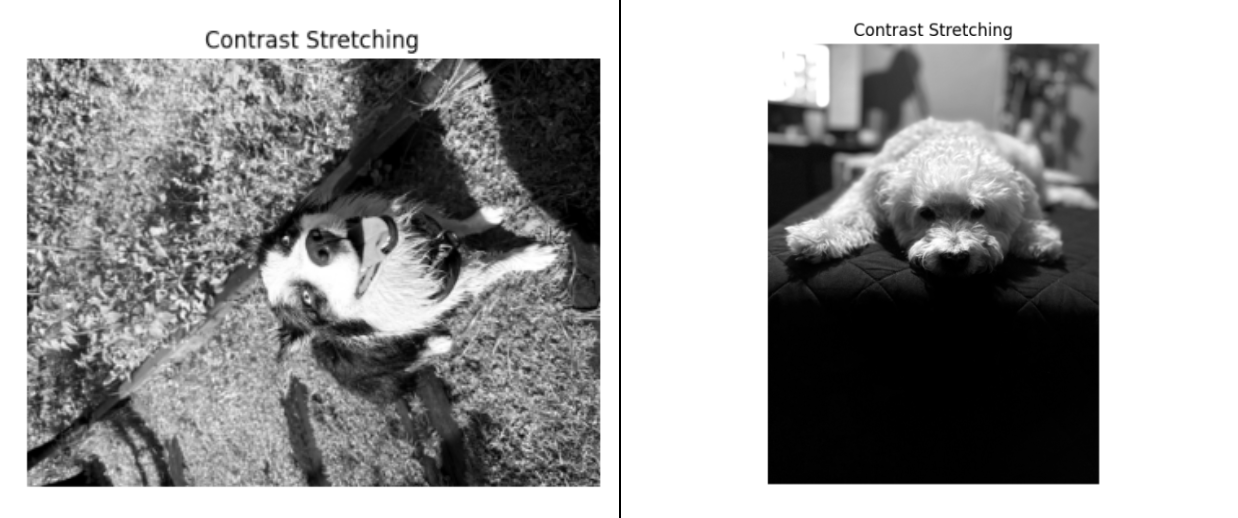
\includegraphics[width=0.8\linewidth]{figuras/estiramiento_de_contraste.png}
  \caption{Aplicación de estiramiento de contraste}
  \label{fig:estiramiento_de_contraste}
\end{figure}

\textbf{Comparativa:} En la Figura \ref{fig:estiramiento_de_contraste_justificacion} se observa que el histograma de la imagen original presenta una concentración de valores en un rango estrecho, mientras que el histograma de la imagen transformada muestra una distribución más amplia y uniforme. Esto evidencia la mejora visual y técnica lograda mediante el estiramiento de contraste.

\begin{figure}[H]
  \centering
  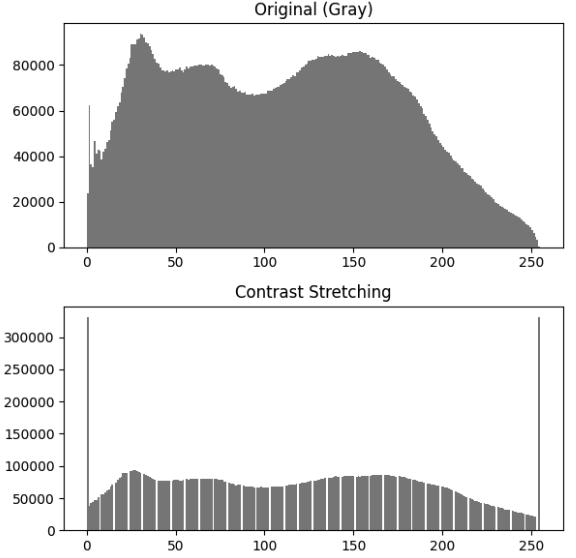
\includegraphics[width=0.8\linewidth]{figuras/estiramiento_de_contraste_justificacion.png}
  \caption{Estiramiento de Contraste: Comparación de histogramas entre imagen original y transformada}
  \label{fig:estiramiento_de_contraste_justificacion}
\end{figure}


\subsubsection{Ecualización del histograma}
La ecualización del histograma es una técnica fotométrica de procesamiento pixel a pixel que redistribuye los valores de intensidad de una imagen para aplanar su histograma. Este proceso mejora el contraste global de la imagen, especialmente en aquellas que presentan una concentración de valores en un rango estrecho, como ocurre en condiciones de iluminación deficiente o en imágenes con bajo rango dinámico.

\textbf{Justificación:} Esta técnica es ampliamente utilizada en aumentación de datos para modelos de inteligencia artificial, ya que permite mejorar la visibilidad de estructuras relevantes en imágenes con bajo contraste. Al redistribuir los valores de intensidad, se facilita la extracción de características por parte de algoritmos de aprendizaje profundo, lo que puede mejorar el desempeño en tareas de clasificación, segmentación o detección.

En este proyecto, se aplicó la ecualización del histograma utilizando la función \texttt{equalizeHist()} de la biblioteca \texttt{cv2}, sobre imágenes previamente convertidas a escala de grises. En la Figura~\ref{fig:ecualizacion_imagen} se observa cómo la ecualización mejora la visibilidad de detalles en imágenes originalmente apagadas, al redistribuir los niveles de intensidad. El siguiente código muestra su implementación:

\begin{minted}{python}
# 3) Histogram equalization
img_eq = cv2.equalizeHist(img1_gray)
\end{minted}

\begin{figure}[H]
  \centering
  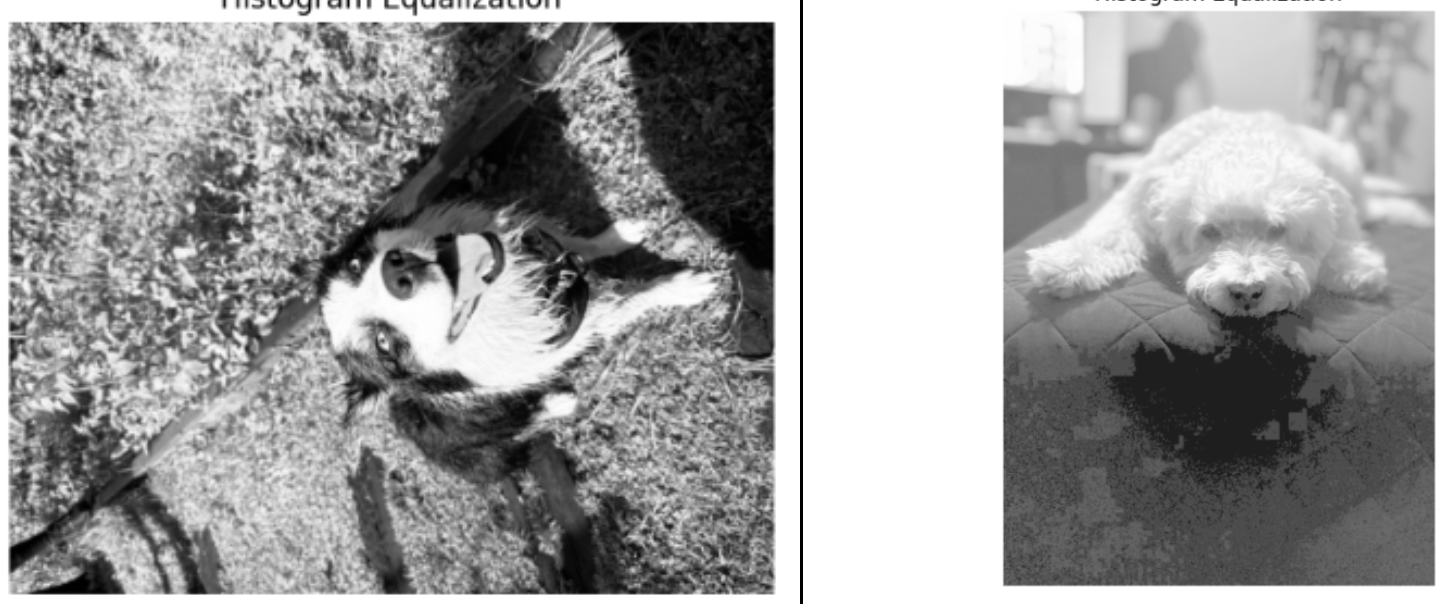
\includegraphics[width=0.8\linewidth]{figuras/ecualizacion_imagen.png}
  \caption{Aplicación de ecualización del histograma sobre imágenes de prueba}
  \label{fig:ecualizacion_imagen}
\end{figure}

\begin{figure}[H]
  \centering
  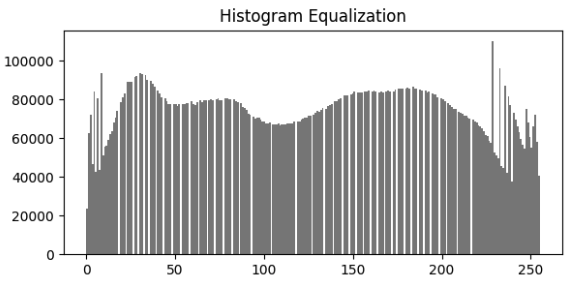
\includegraphics[width=0.8\linewidth]{figuras/ecualizacion_histograma.png}
  \caption{Histograma resultante tras aplicar ecualización}
  \label{fig:ecualizacion_histograma}
\end{figure}


\textbf{Comparativa e interpretación del histograma:} Como se observa en la Figura~\ref{fig:ecualizacion_histograma}, el histograma original presentaba una concentración de valores en un rango limitado, lo que se traduce en una imagen visualmente apagada. Tras aplicar la ecualización, los valores se distribuyen de forma más uniforme en el rango de 0 a 255, lo que mejora significativamente el contraste y la percepción de detalles. Esta redistribución permite que los modelos de visión computacional trabajen con imágenes más informativas.

\subsubsection{Comparativa de Histogramas de las transformaciones}
Para evaluar el impacto de las transformaciones fotométricas aplicadas (transformación logarítmica, estiramiento de contraste y ecualización del histograma) se realizó una comparativa visual de los histogramas resultantes. Esta comparación permite observar cómo cada técnica modifica la distribución de los niveles de intensidad en las imágenes, lo cual se traduce en mejoras perceptibles en el contraste y la visibilidad de detalles.

\begin{figure}[H]
  \centering
  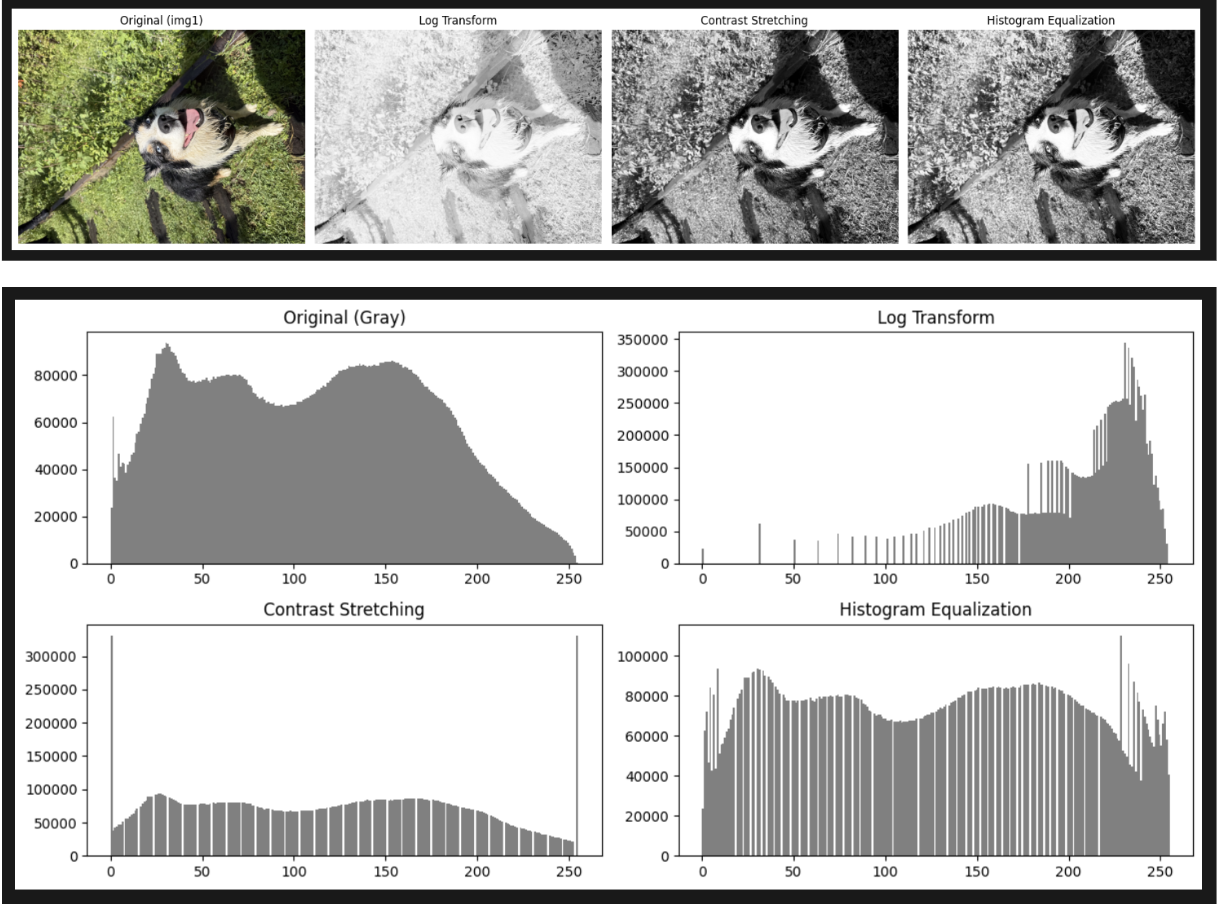
\includegraphics[width=0.8\linewidth]{figuras/comparacion_transformaciones.png}
  \caption{Comparación de imágenes y sus histogramas tras aplicar transformaciones fotométricas}
  \label{fig:comparacion_transformaciones}
\end{figure}

\textbf{Interpretación:} En la Figura~\ref{fig:comparacion_transformaciones} se observa que:

\begin{itemize}
    \item El histograma de la imagen original presenta una concentración de valores en un rango estrecho, lo que indica bajo contraste.
    \item La transformación logarítmica expande los valores bajos hacia el centro del histograma, mejorando la visibilidad en zonas oscuras.
    \item El estiramiento de contraste redistribuye los valores de forma más amplia, extendiendo el rango dinámico sin alterar la forma general del histograma.
    \item La ecualización del histograma genera una distribución más uniforme en todo el rango de 0 a 255, lo que resulta en un contraste más equilibrado y una imagen visualmente más clara.
\end{itemize}

Esta comparativa confirma que cada técnica tiene un efecto distinto sobre la imagen, y su elección depende del tipo de mejora deseada. En el contexto de aumentación de datos para inteligencia artificial, estas transformaciones permiten generar variantes útiles de las imágenes originales, enriqueciendo el conjunto de entrenamiento y mejorando la capacidad de generalización de los modelos.

\subsection{Negativo de Imagen}

La inversión de una imagen, o la obtención de su negativo, es una transformación a nivel de píxel donde la intensidad de cada píxel se resta del valor de intensidad máximo posible. Esta técnica es de gran valor en el análisis de películas de radiología, ya que puede hacer que los detalles de bajo contraste sean más visibles.

En las películas de rayos X tradicionales, los huesos y tejidos densos aparecen como áreas claras sobre un fondo oscuro. Para este ejercicio, el uso de esta técnica para la detección de billetes falsos resulta altamente conveniente, pues resalta detalles difíciles de detectar a simple vista. Las Figuras \ref{fig:billete_original_anverso} y \ref{fig:billete_original_reverso} muestran el anverso y reverso de un billete de 500 pesos mexicanos antes de realizar la transformación.

\textbf{Justificación:} El uso de la inversión de imágenes para el análisis de billetes falsos se justifica por la manera en que esta técnica resalta características de seguridad que son difíciles de ver a simple vista. Los billetes auténticos contienen marcas de agua, hilos de seguridad y microimpresiones diseñadas para ser sutiles y difíciles de replicar.

\textbf{Demostración:} Al invertir la imagen, los detalles de los billetes que son difíciles de ver a simple vista se vuelven más evidentes como se puede apreciar en las Figuras \ref{fig:billete_negativo_1} y \ref{fig:billete_negativo_2}. Las marcas de seguridad o texturas que eran claras se vuelven oscuras y viceversa.
Este contraste mejorado facilita que los sistemas de visión computacional y las máquinas de detección identifiquen y validen estas características, permitiendo una verificación rápida y precisa de la autenticidad del billete.

\begin{figure}[H]
  \centering
  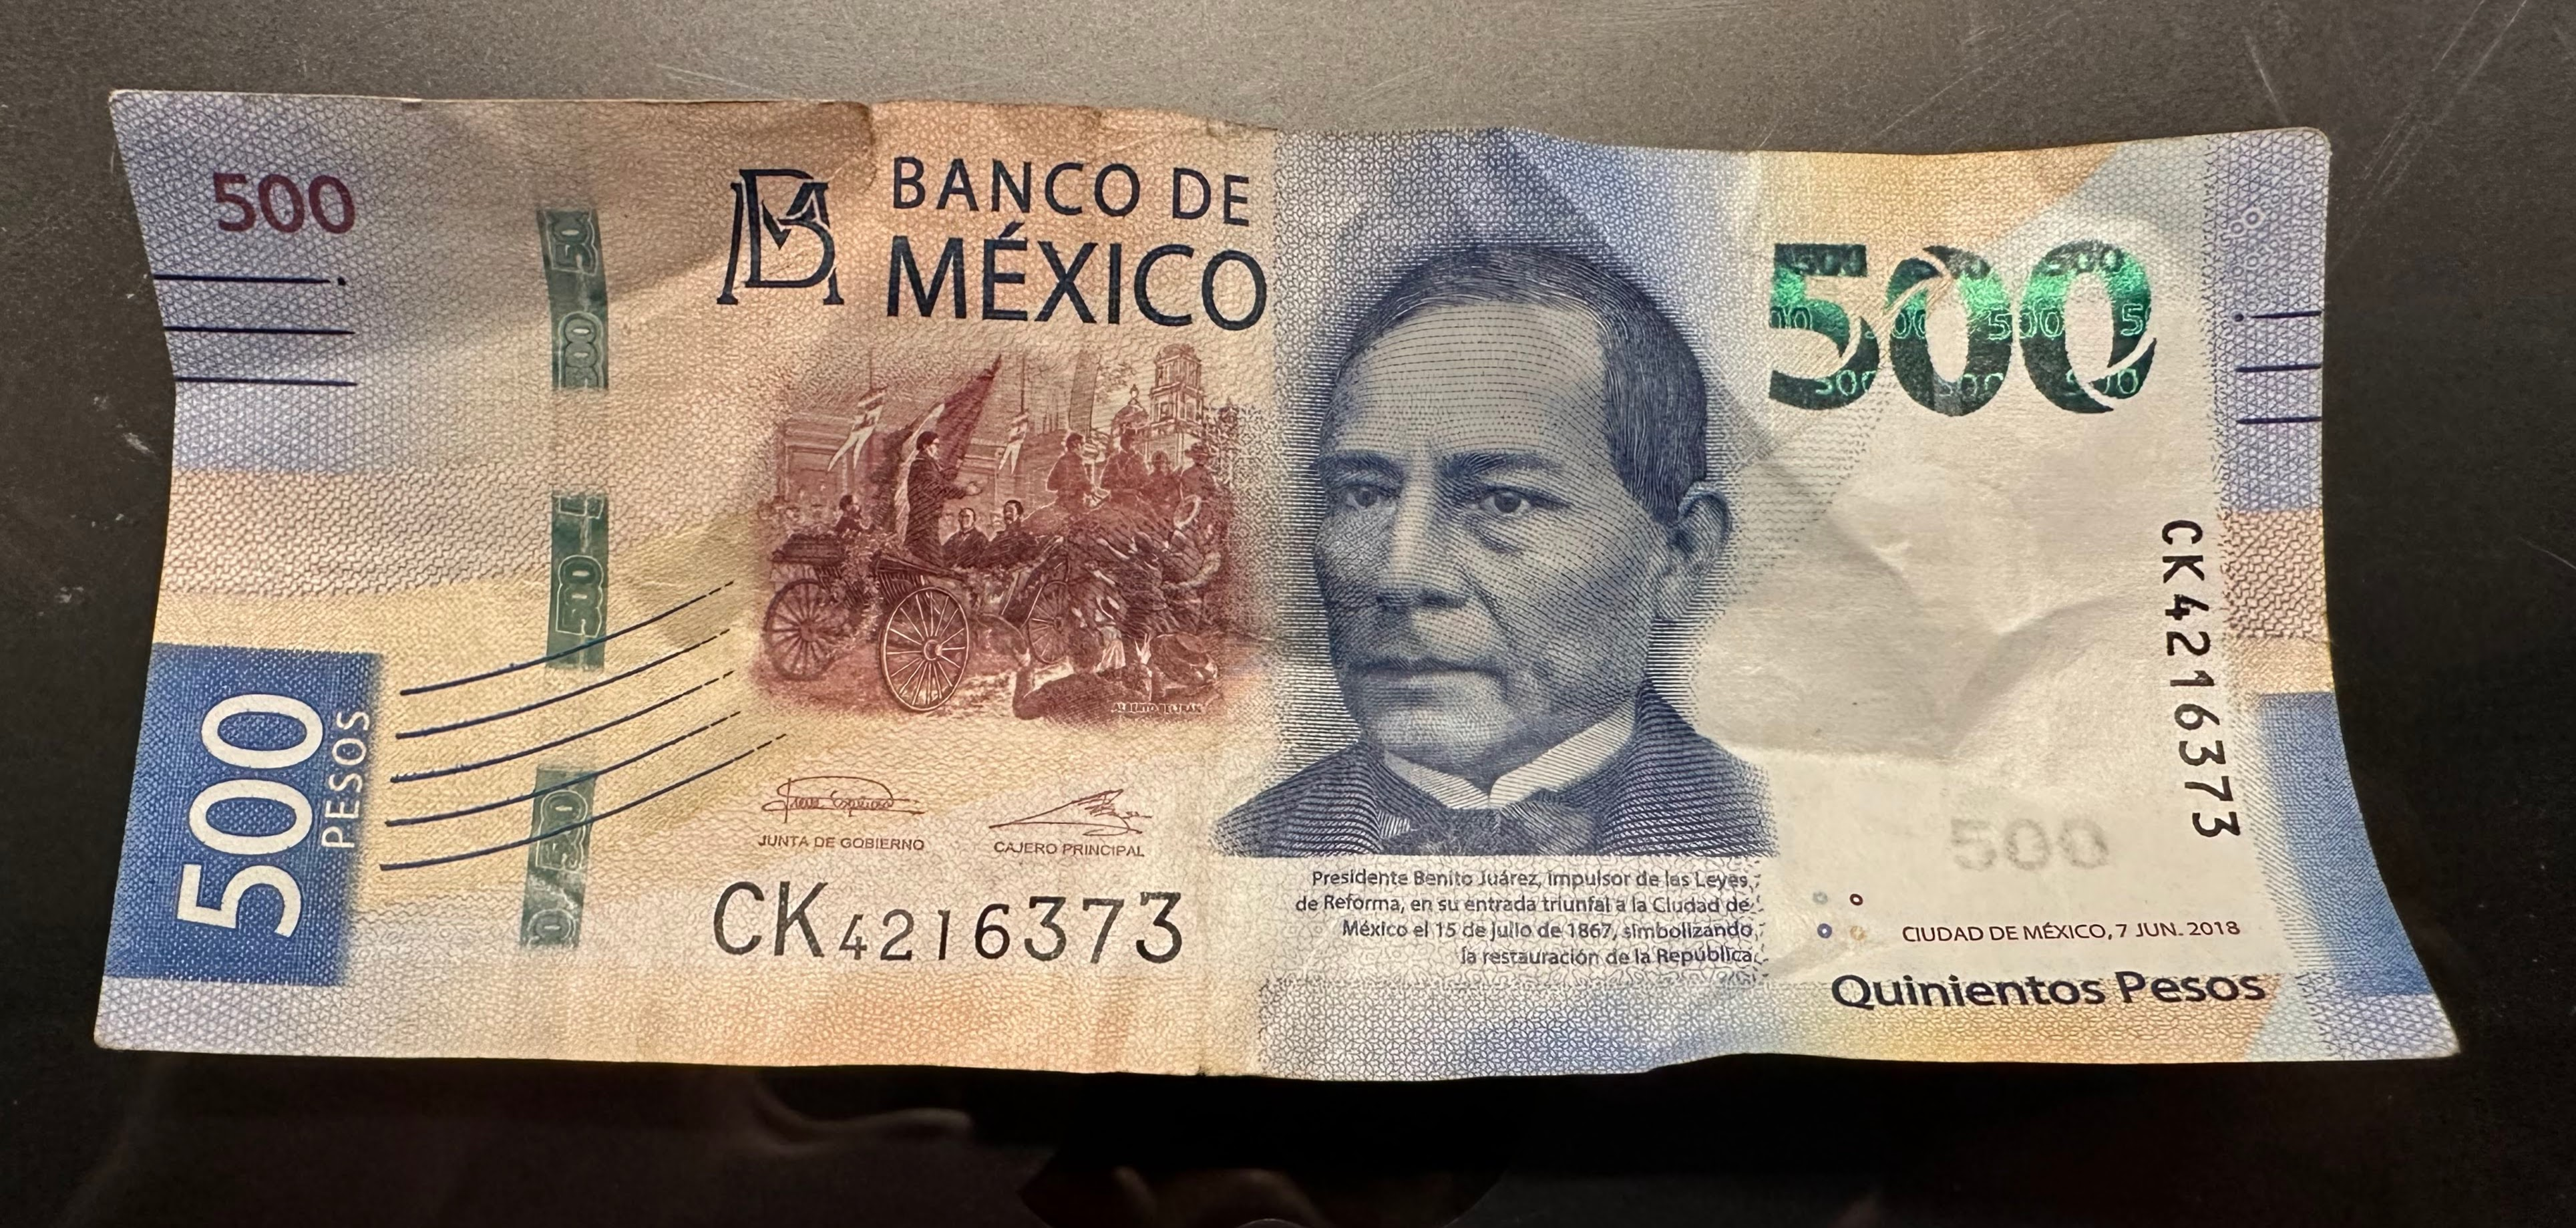
\includegraphics[width=0.5\linewidth]{../data/billete-original/img2.jpg}
  \caption{Billete Original: Anverso}
  \label{fig:billete_original_anverso}
\end{figure}

\begin{figure}[H]
  \centering
  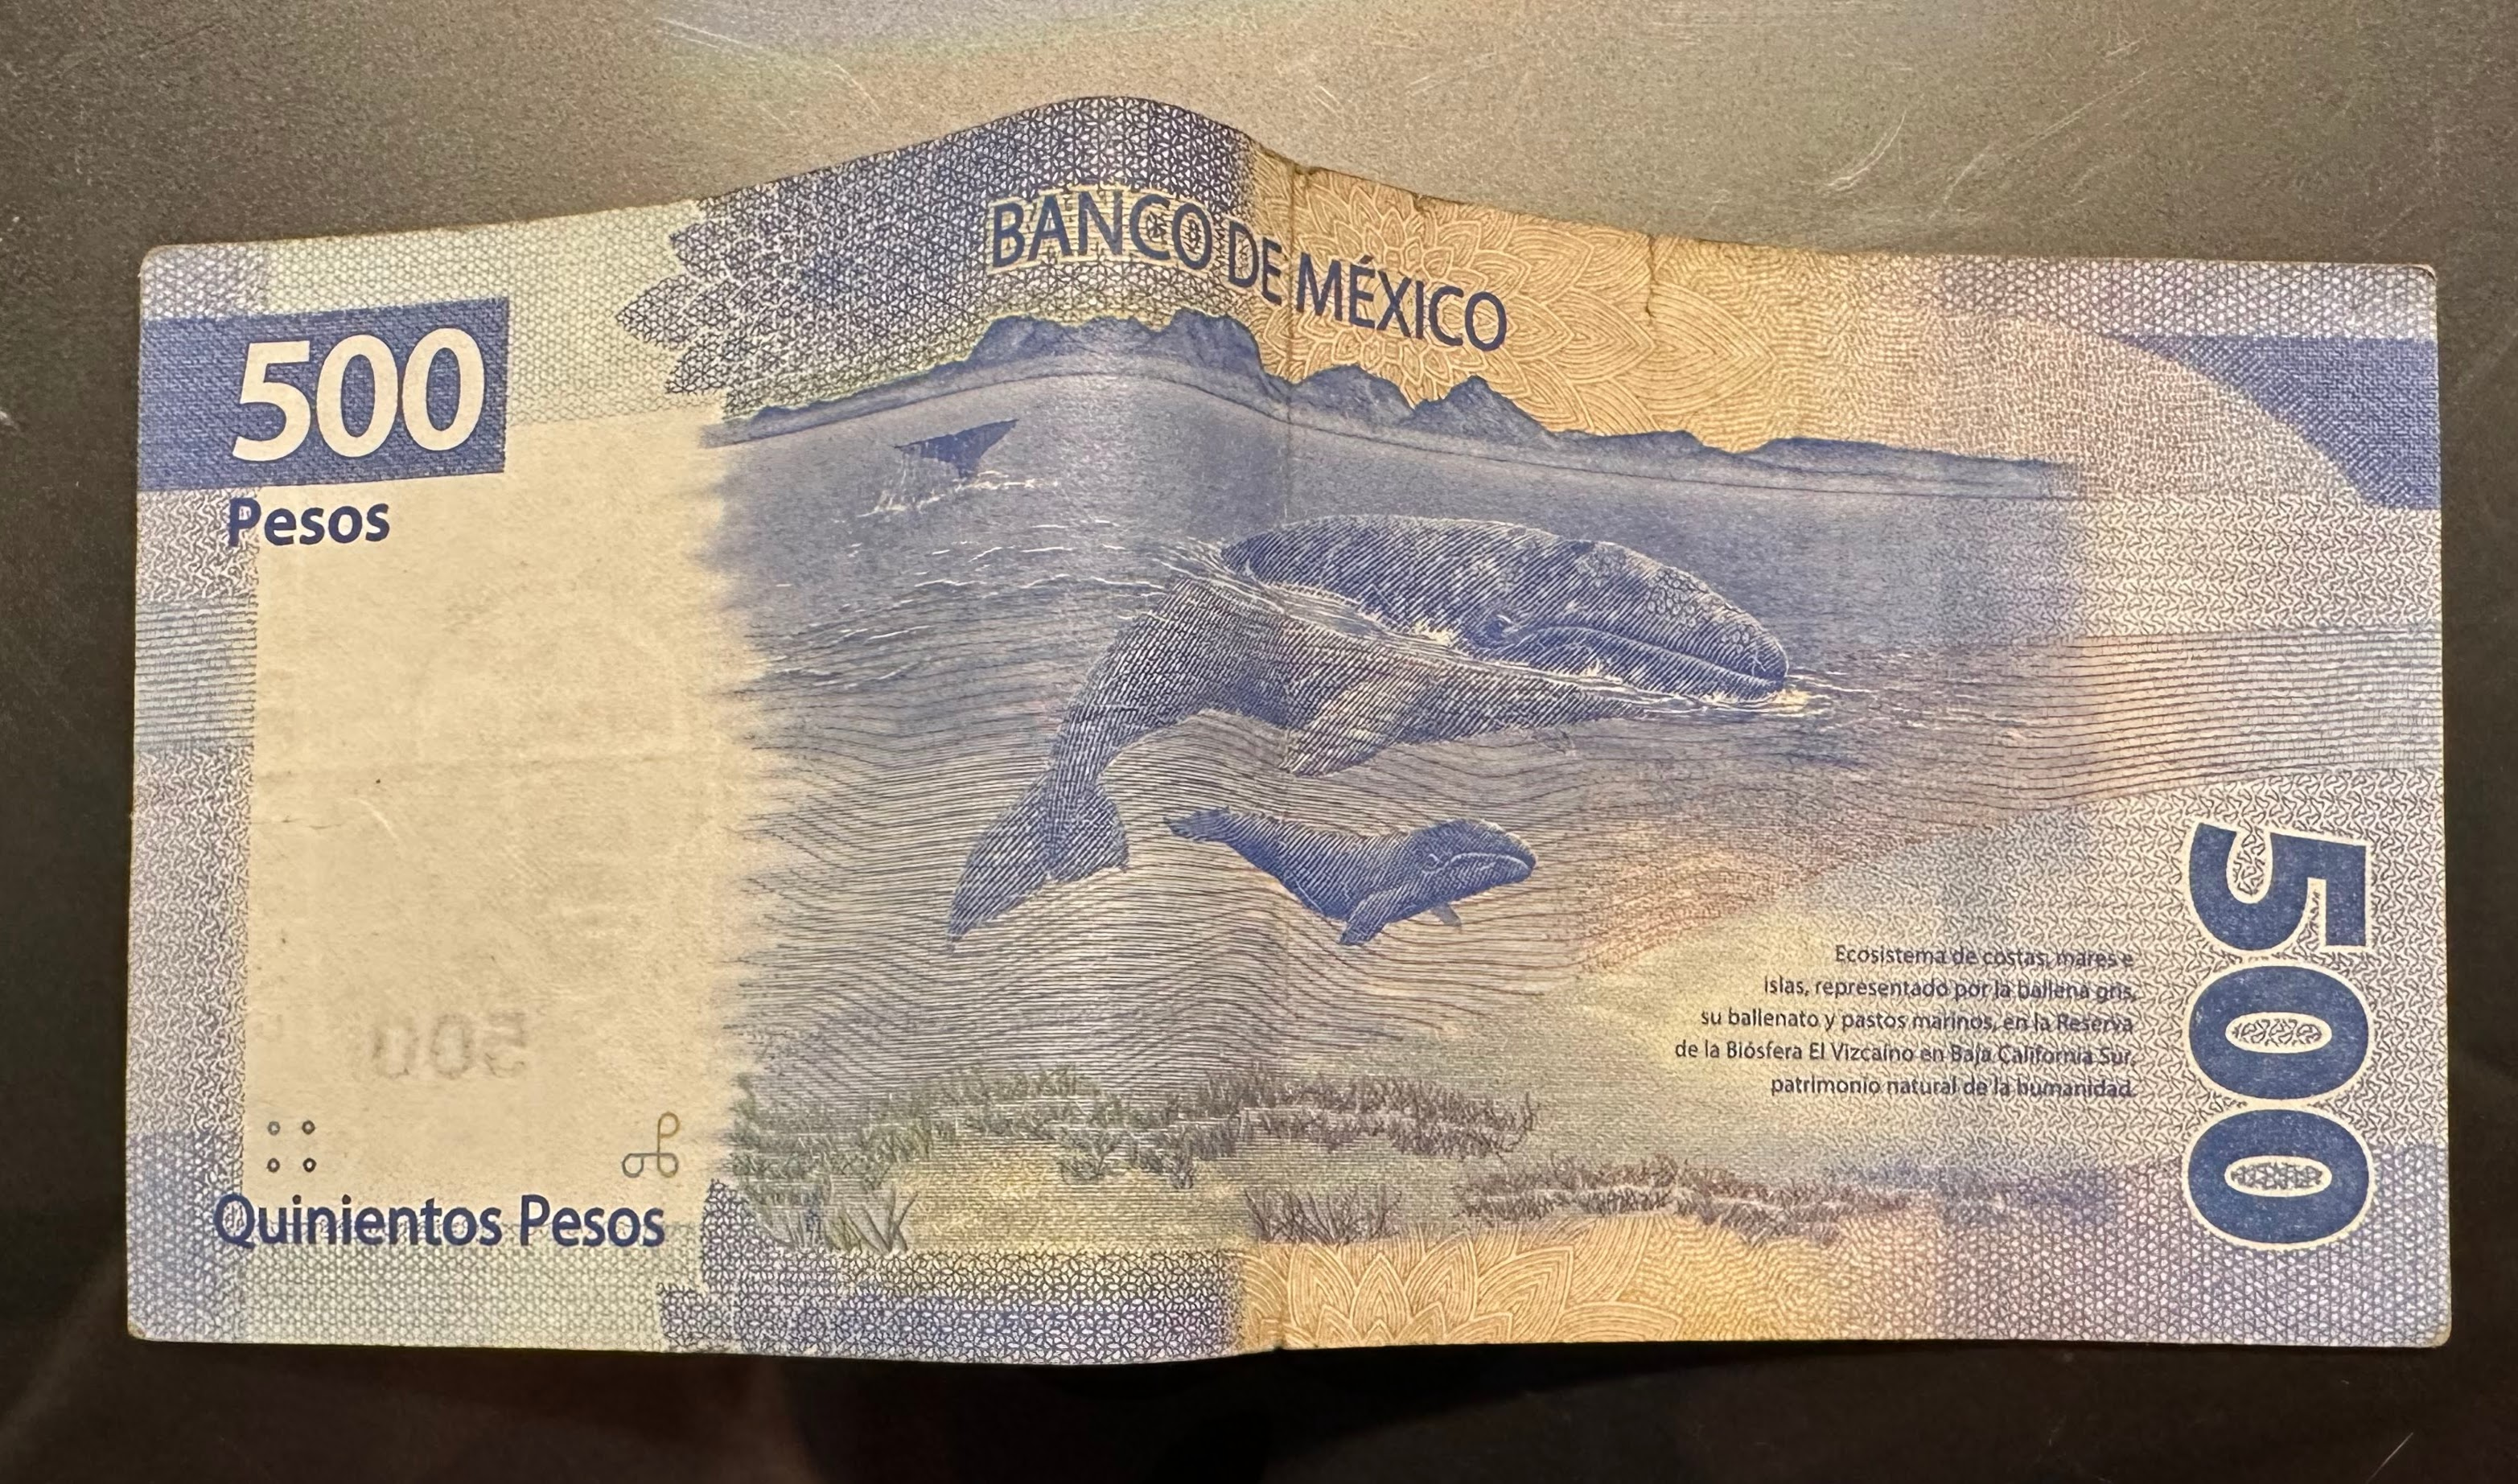
\includegraphics[width=0.5\linewidth]{../data/billete-original/img1.jpg}
  \caption{Billete Original: Reverso}
  \label{fig:billete_original_reverso}
\end{figure}


El siguiente código muestra como se puede aplicar dicha transformación:

\begin{minted}{python}
bill1 = mpimg.imread('data/billete-original/img1.jpg')
bill2 = mpimg.imread('data/billete-original/img2.jpg')

neg_bill1 = cv2.bitwise_not(bill1)
neg_bill2 = cv2.bitwise_not(bill2)

# Show in a 2x2 grid: original and negative for each bill
fig, axes = plt.subplots(2, 2, figsize=(12, 10))

axes[0, 0].imshow(bill1)
axes[0, 0].set_title('Bill 1 - Original')
axes[0, 0].axis('off')

axes[0, 1].imshow(neg_bill1)
axes[0, 1].set_title('Bill 1 - Negative')
axes[0, 1].axis('off')

axes[1, 0].imshow(bill2)
axes[1, 0].set_title('Bill 2 - Original')
axes[1, 0].axis('off')

axes[1, 1].imshow(neg_bill2)
axes[1, 1].set_title('Bill 2 - Negative')
axes[1, 1].axis('off')
plt.tight_layout()
plt.show()
# Grayscale histogram for each bill and its negative
def plot_gray_hist(ax, image, title):
    gray = cv2.cvtColor(image, cv2.COLOR_RGB2GRAY)
    ax.hist(gray.ravel(), bins=256, range=(0,256), color='black')
    ax.set_title(title)
    ax.set_xlim(0,256)

fig, axes = plt.subplots(2, 2, figsize=(12, 8))

plot_gray_hist(axes[0, 0], bill1, 'Bill 1 - Histogram (Original)')
plot_gray_hist(axes[0, 1], neg_bill1, 'Bill 1 - Histogram (Negative)')
plot_gray_hist(axes[1, 0], bill2, 'Bill 2 - Histogram (Original)')
plot_gray_hist(axes[1, 1], neg_bill2, 'Bill 2 - Histogram (Negative)')

plt.tight_layout()
plt.show()
\end{minted}

\begin{figure}[H]
  \centering
  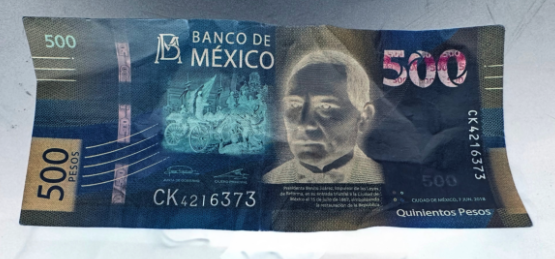
\includegraphics[width=0.5\linewidth]{figuras/negativo1.png}
  \caption{Negativo de Imagen: Anverso}
  \label{fig:billete_negativo_1}
\end{figure}

\begin{figure}[H]
  \centering
  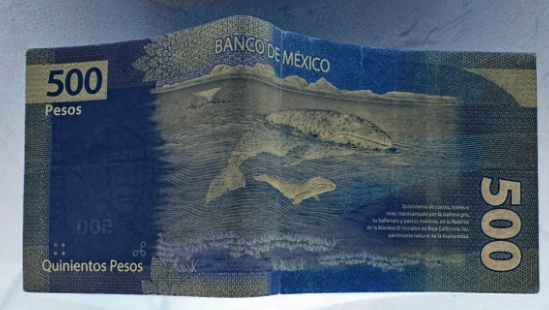
\includegraphics[width=0.5\linewidth]{figuras/negativo2.png}
  \caption{Negativo de Imagen: Reverso}
  \label{fig:billete_negativo_2}
\end{figure}

\begin{figure}[H]
  \centering
  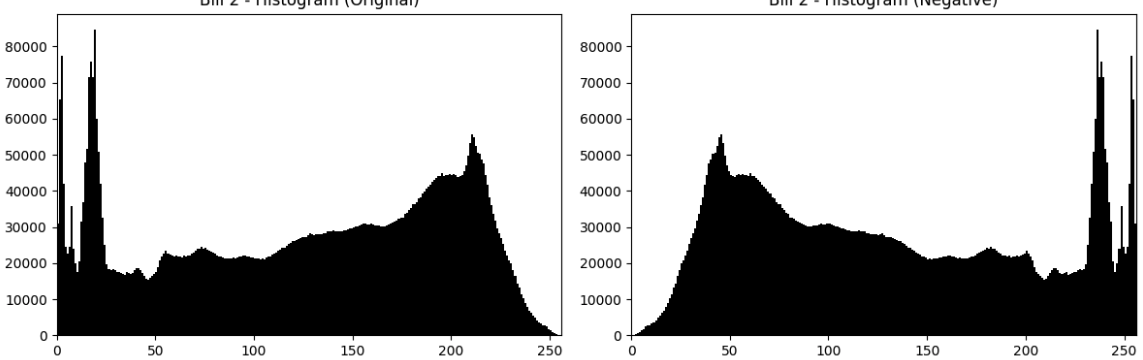
\includegraphics[width=0.5\linewidth]{figuras/histograma_negativo1.png}
  \caption{Histogramas Anverso}
  \label{fig:histograma_negativo1}
\end{figure}

\begin{figure}[H]
  \centering
  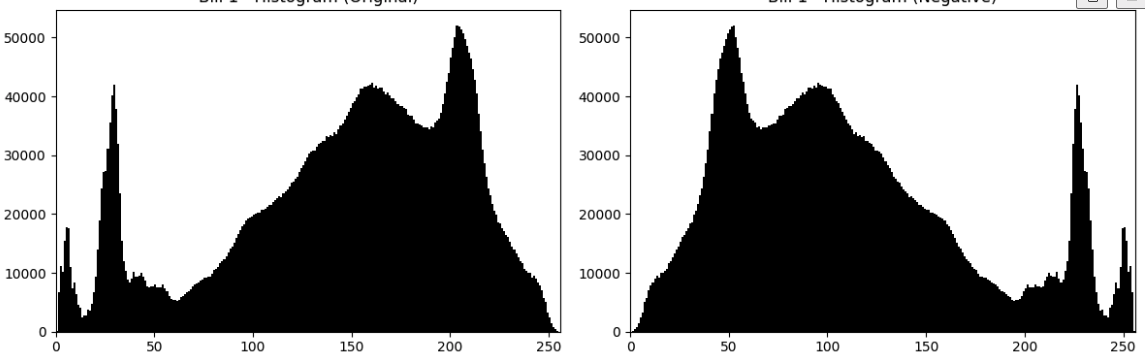
\includegraphics[width=0.5\linewidth]{figuras/histograma_negativo2.png}
  \caption{Histogramas Reverso}
  \label{fig:histograma_negativo2}
\end{figure}


\textbf{Análisis del Histograma:} Los histogramas de los billetes originales y sus negativos son inversos. Los picos de intensidad que estaban en el lado derecho (brillante) del histograma original se mueven al lado izquierdo (oscuro) en el histograma negativo, y viceversa. Esto refleja el cambio de luminancia en la imagen. En las Figuras \ref{fig:histograma_negativo1} y \ref{fig:histograma_negativo2} se muestra la comparativa de los histogramas de las imágenes originales (lado derecho) con el histograma de su contraparte negativa (lado izquierdo), del anverso y reverso del billete, respectivamente.

\subsection{Corrección de Gamma}

La corrección de gamma es una operación no lineal utilizada para codificar o decodificar la luminancia en las imágenes. 

\textbf{Justificación:} Es especialmente útil en campos como la astronomía, donde ayuda a equilibrar la representación visual de objetos celestes muy brillantes y muy oscuros.
En las imágenes astronómicas, los objetos tenues como las nebulosas y las galaxias distantes tienen valores de píxel muy bajos en comparación con las estrellas brillantes. Un valor de gamma menor que 1 ($\gamma < 1$) ilumina los tonos medios y las sombras, haciendo que los detalles tenues sean más visibles sin saturar las estrellas brillantes. Por el contrario, un valor de gamma mayor que 1 ($\gamma > 1$) oscurece la imagen, lo que puede usarse para reducir el ruido de fondo.

\textbf{Demostración:} El siguiente código crea una función que aplica la Corrección Gamma:

\begin{minted}{python}
def apply_gamma(image_gray, gamma):
    invGamma = 1.0 / gamma
    table = np.array([((i / 255.0) ** invGamma) * 255 for i in np.arange(256)]).astype("uint8")
    return cv2.LUT(image_gray, table)

# List of gammas to test (adjust as needed)
gammas = [0.3, 0.5, 0.7, 0.9, 1.0, 1.2, 1.5, 2.0]
results = [(g, apply_gamma(imgPopo, g)) for g in gammas]

# Show original + corrections in a 3x3 grid
fig, axes = plt.subplots(3, 3, figsize=(12, 12))
axes = axes.ravel()

# Position 0: Original
axes[0].imshow(imgPopo, cmap='gray')
axes[0].set_title('Original')
axes[0].axis('off')

# Rest: different gammas
for ax, (g, img_c) in zip(axes[1:], results):
    ax.imshow(img_c, cmap='gray')
    ax.set_title(f'gamma={g}')
    ax.axis('off')

# Hide extra axes if any
for k in range(1 + len(results), len(axes)):
    axes[k].axis('off')

plt.tight_layout()
plt.show()
\end{minted}


\begin{figure}[H]
  \centering
  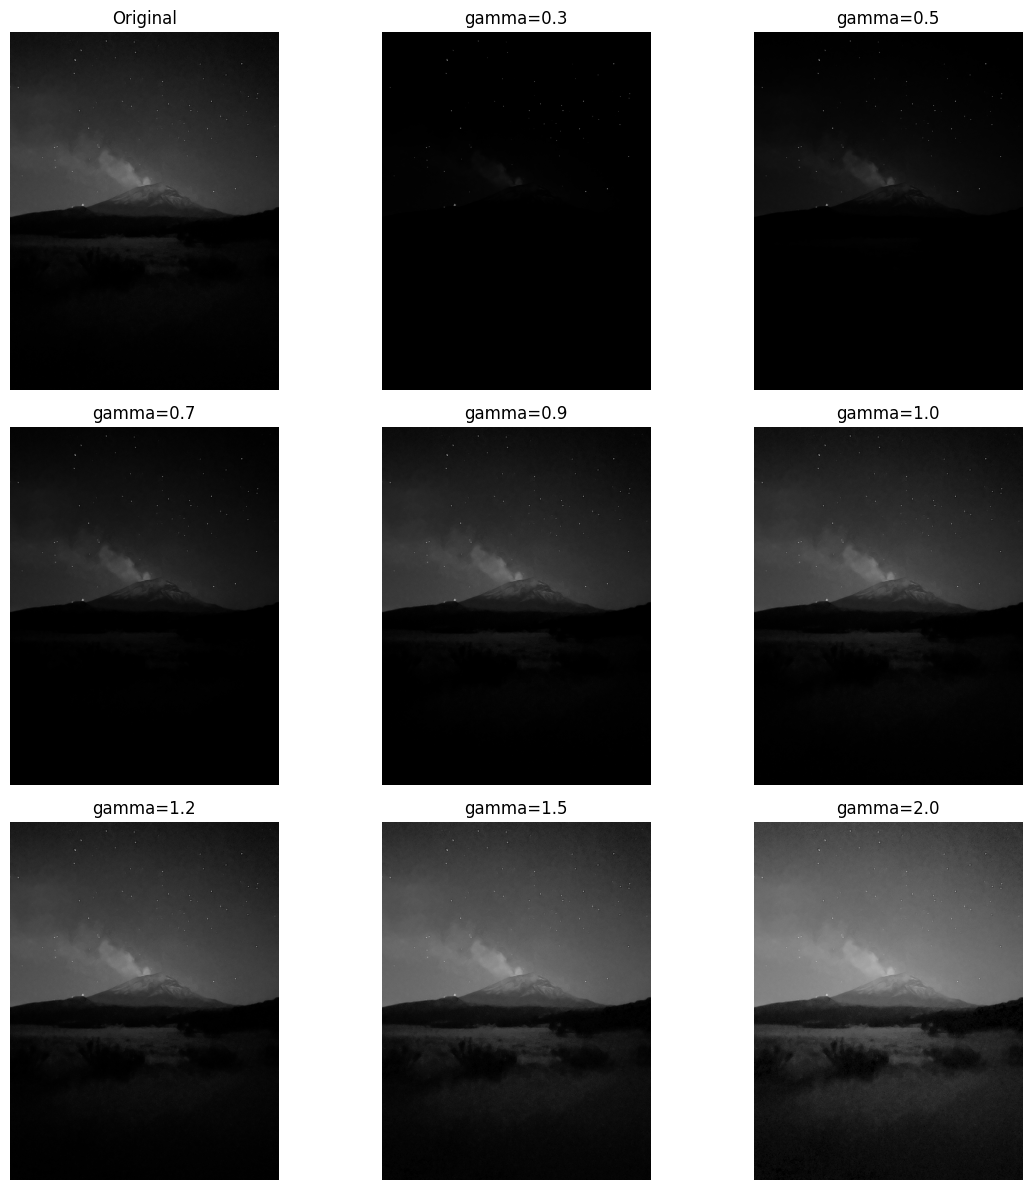
\includegraphics[width=0.5\linewidth]{figuras/correccion_gamma.png}
  \caption{Corrección Gamma: Múltiples transformaciones}
  \label{fig:correccion_gamma}
\end{figure}

La Figura \ref{fig:correccion_gamma} muestra diferentes imágenes producidas variando los valores de $\gamma$, donde se puede observar lo siguiente:

\begin{itemize}
  \item \textbf{$\gamma < 1$}: La imagen se vuelve progresivamente más brillante. Los tonos medios y las sombras se iluminan, haciendo que los detalles tenues sean más visibles sin saturar las partes brillantes.
  \item \textbf{$\gamma > 1$}: La imagen se oscurece. Los tonos medios se vuelven más oscuros, lo que puede ser útil para reducir el ruido de fondo.
  \item \textbf{$\gamma = 1$}: La imagen permanece sin cambios, sirviendo como el punto de referencia.
\end{itemize}

\subsection{Sustracción de Imágenes}

La sustracción de imágenes es una técnica para detectar cambios entre dos imágenes capturadas en momentos diferentes pero desde el mismo punto de vista. 

\textbf{Justificación:} Se aplica ampliamente en la vigilancia de seguridad para detectar movimiento o la aparición de nuevos objetos en una escena.
Al restar una imagen de fondo de referencia de un nuevo fotograma, cualquier valor de píxel que no sea cero representa un cambio. Este método crea una máscara  de cambio que aísla los objetos en movimiento del fondo estático. Después de un simple umbral y operaciones morfológicas para limpiar el ruido, la máscara de cambio se puede usar para identificar y localizar intrusos u otros eventos significativos, convirtiéndose en un método potente y de bajo costo para sistemas de monitoreo en tiempo real.

\textbf{Demostración:} En nuestro ejemplo, las figuras \ref{fig:sustraccion_referencia} y \ref{fig:sustraccion_actual} representan la imagen de referencia e imagen actual respectivamente.

\begin{figure}[H]
  \centering
  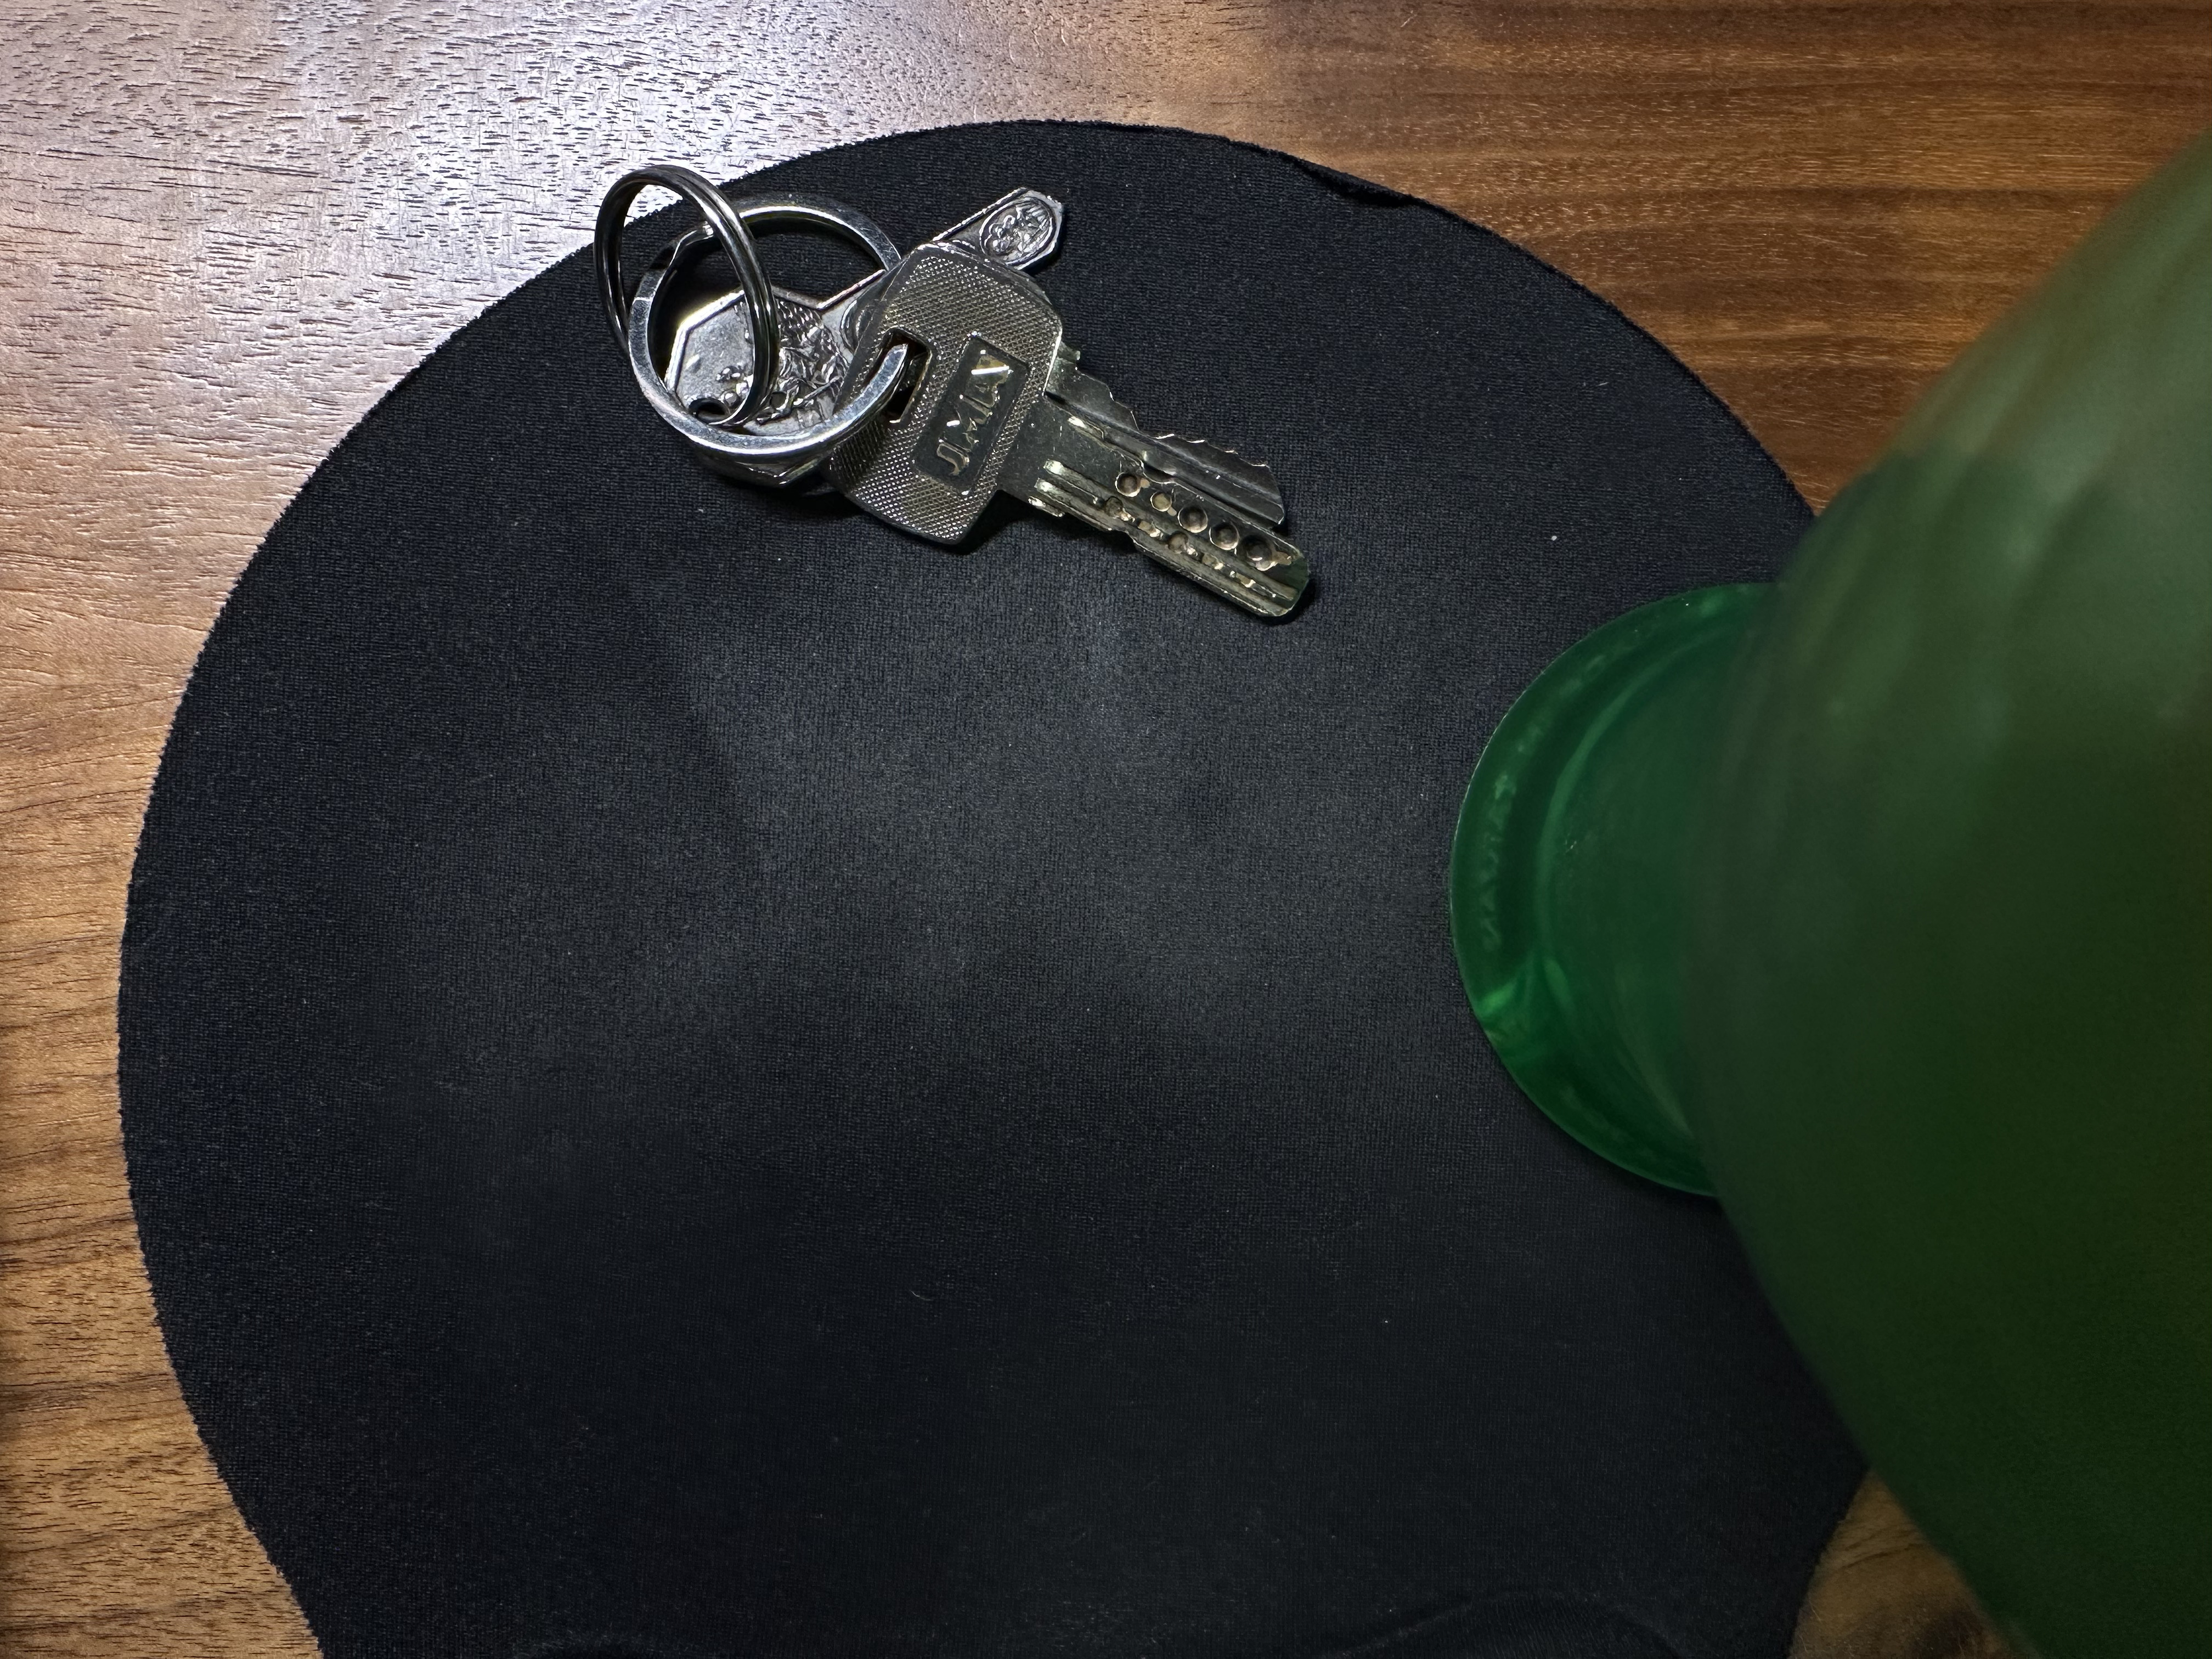
\includegraphics[width=0.5\linewidth]{../data/data-substraction-sample/img-1.jpg}
  \caption{Sustracción de Imágenes: Imagen de Referencia}
  \label{fig:sustraccion_referencia}
\end{figure}

\begin{figure}[H]
  \centering
  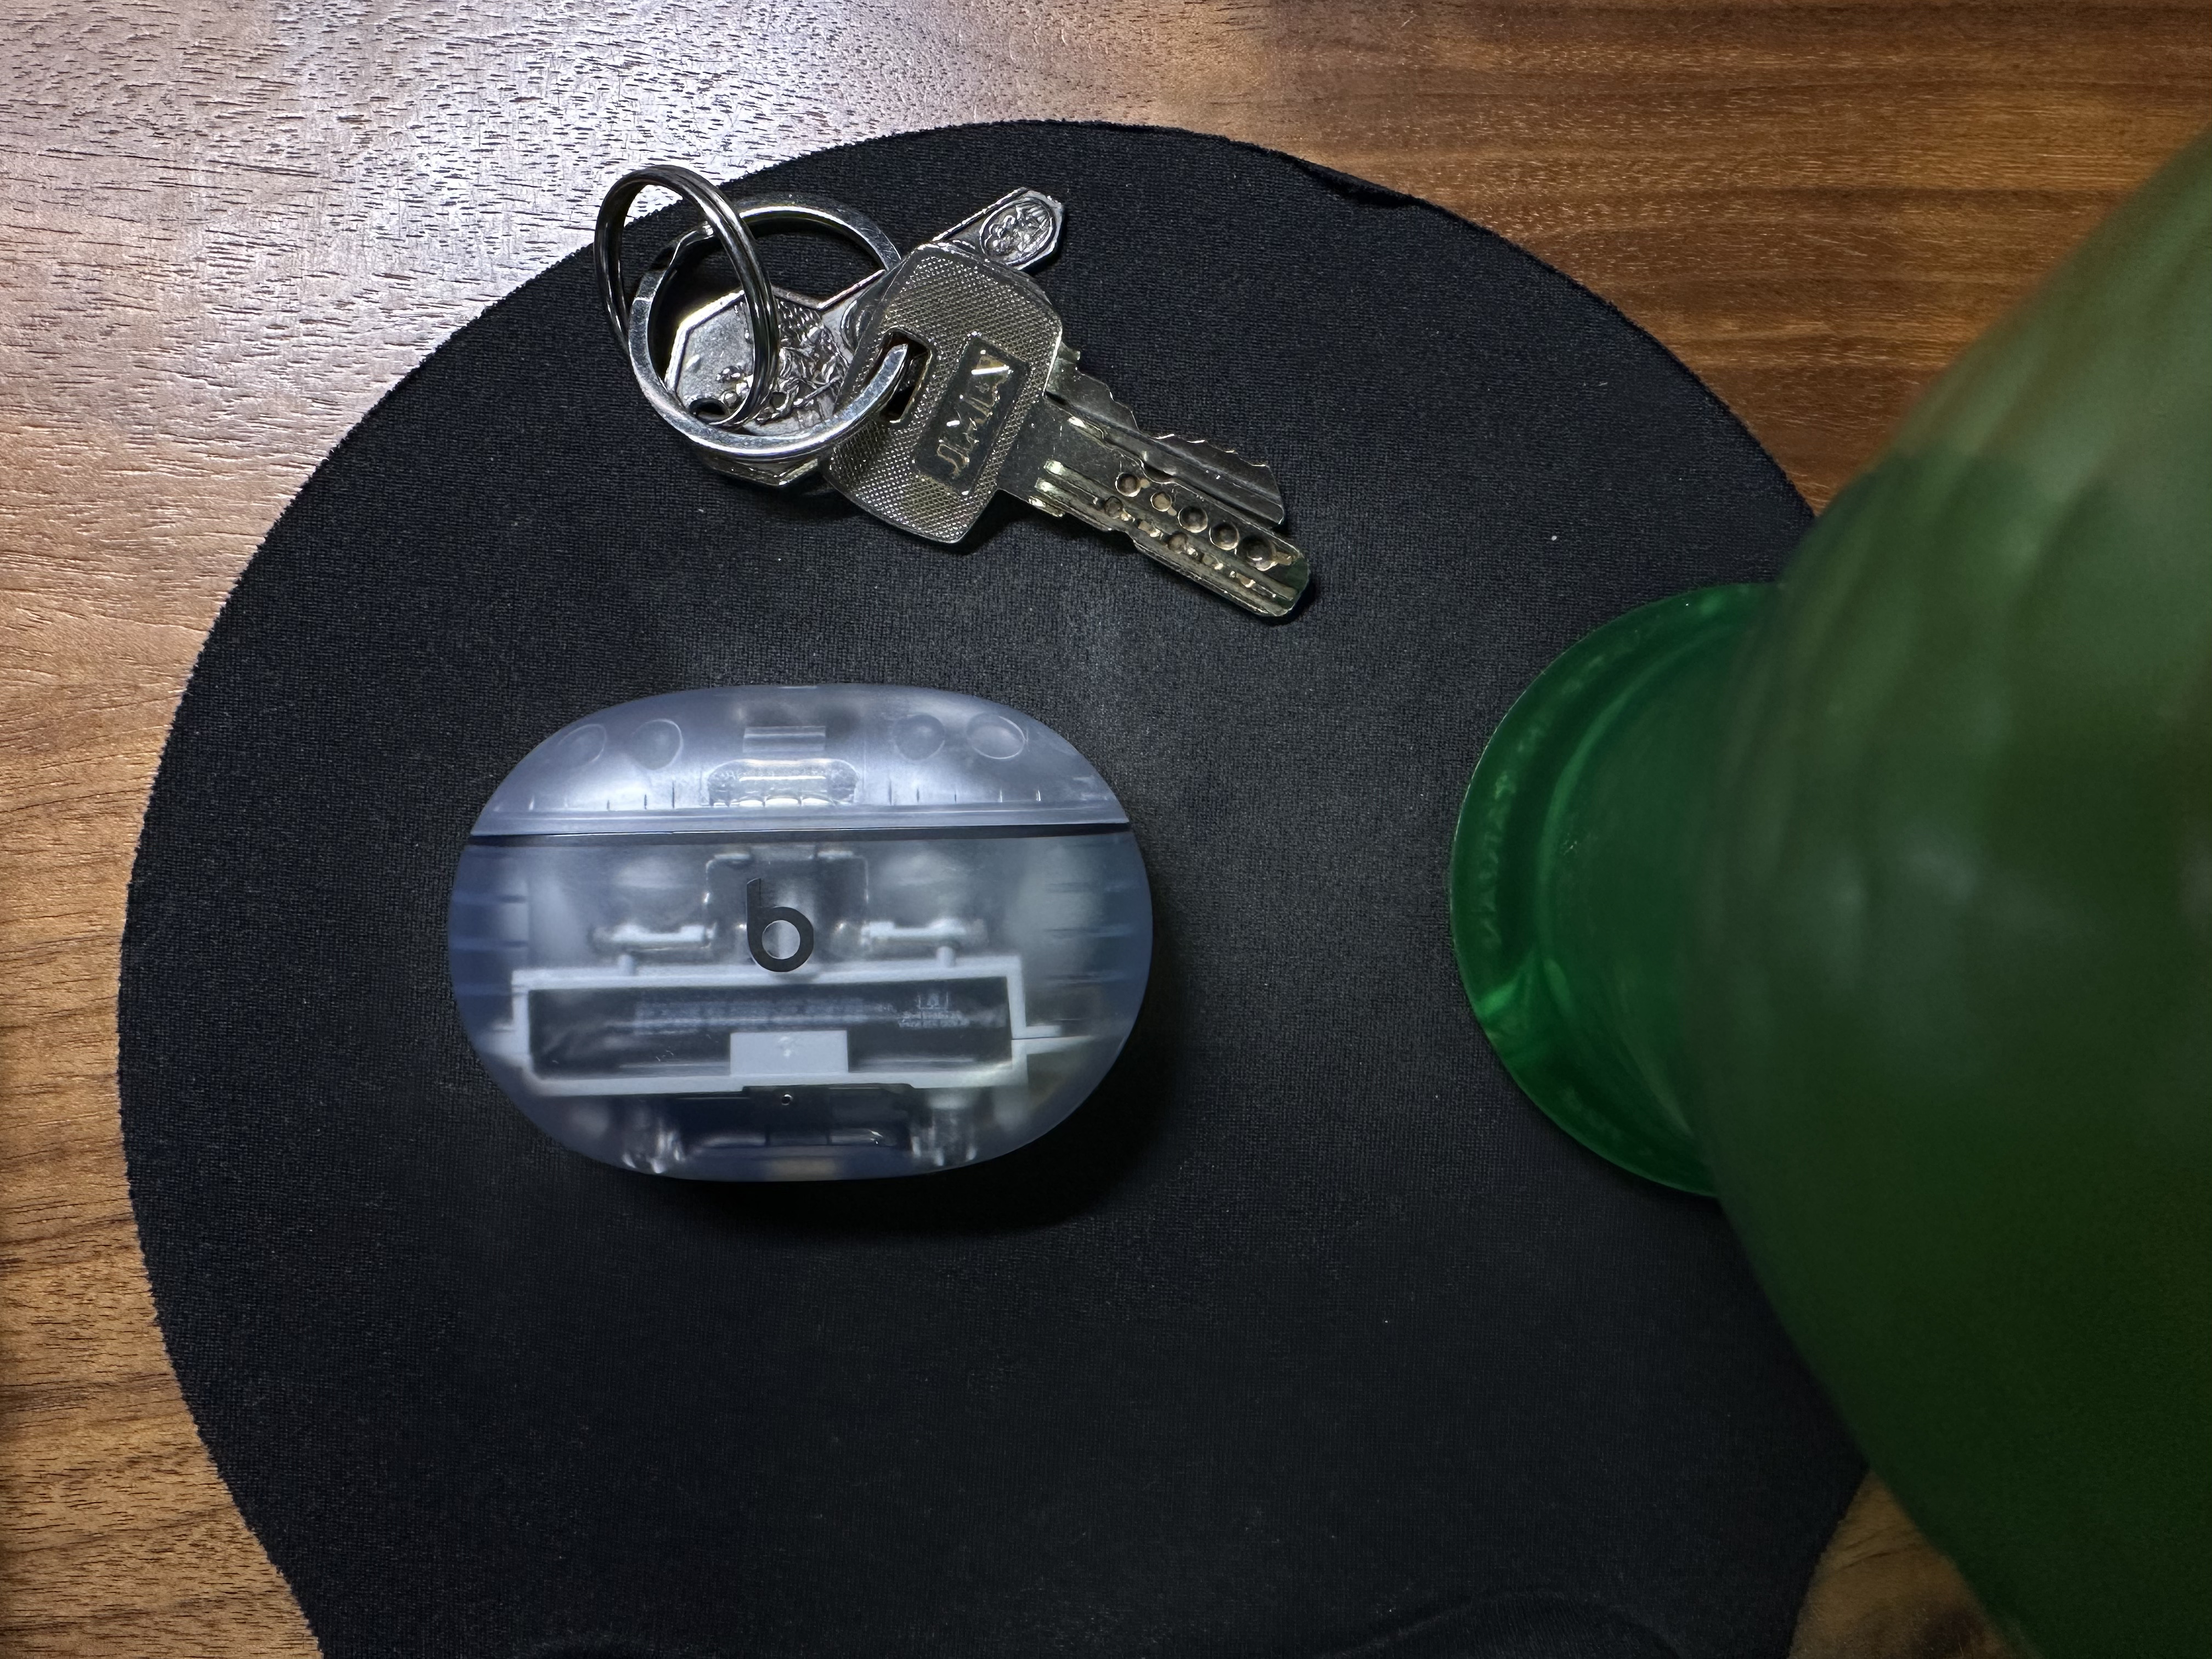
\includegraphics[width=0.5\linewidth]{../data/data-substraction-sample/img-2.jpg}
  \caption{Sustracción de Imágenes: Imagen actual}
  \label{fig:sustraccion_actual}
\end{figure}

El siguiente código nos permite realizar la sustracción de imágenes y detectar los objetos nuevos:


\begin{minted}{python}
imgV1 = mpimg.imread('data/data-substraction-sample/img-1.jpg')
imgV2 = mpimg.imread('data/data-substraction-sample/img-2.jpg')

# Ensure both images have the same shape for subtraction
if imgV1.shape != imgV2.shape:
    # Resize the second image to match the first
    imgV2_resized = cv2.resize(imgV2, (imgV1.shape[1], imgV1.shape[0]))
else:
    imgV2_resized = imgV2

# Convert to grayscale for better processing
if imgV1.ndim == 3:
    gray1 = cv2.cvtColor(imgV1, cv2.COLOR_RGB2GRAY)
else:
    gray1 = imgV1

if imgV2_resized.ndim == 3:
    gray2 = cv2.cvtColor(imgV2_resized, cv2.COLOR_RGB2GRAY)
else:
    gray2 = imgV2_resized

# Ensure 8-bit
if gray1.dtype != np.uint8:
    gray1 = cv2.normalize(gray1, None, 0, 255, cv2.NORM_MINMAX).astype(np.uint8)
if gray2.dtype != np.uint8:
    gray2 = cv2.normalize(gray2, None, 0, 255, cv2.NORM_MINMAX).astype(np.uint8)

# Detect NEW objects: objects that appear in img2 but not in img1
# Method: Find regions where img2 is significantly brighter than img1
diff_new = cv2.subtract(gray2, gray1)  # Only positive differences (new objects)

# Apply threshold to isolate new objects
_, mask_new = cv2.threshold(diff_new, 30, 255, cv2.THRESH_BINARY)  # Adjust threshold as needed

# Morphological operations to clean up the mask
kernel = np.ones((5, 5), np.uint8)
mask_clean = cv2.morphologyEx(mask_new, cv2.MORPH_OPEN, kernel, iterations=2)
mask_clean = cv2.morphologyEx(mask_clean, cv2.MORPH_CLOSE, kernel, iterations=3)

# Find contours of new objects
contours, _ = cv2.findContours(mask_clean, cv2.RETR_EXTERNAL, cv2.CHAIN_APPROX_SIMPLE)

# Filter and draw bounding boxes for new objects
vis = imgV2_resized.copy()
if vis.ndim == 2:
    vis = cv2.cvtColor(vis, cv2.COLOR_GRAY2RGB)

new_objects = []
for c in contours:
    x, y, w, h = cv2.boundingRect(c)
    area = w * h
    if area < 100:  # Filter out very small objects
        continue
    new_objects.append((x, y, w, h))
    cv2.rectangle(vis, (x, y), (x + w, y + h), (0, 255, 0), 2)  # Green for new objects
    cv2.putText(vis, f'New {len(new_objects)}', (x, y-10), cv2.FONT_HERSHEY_SIMPLEX, 0.7, (0, 255, 0), 2)

# Summary metrics for new objects only
num_new_objects = len(new_objects)
areas = [w * h for (_, _, w, h) in new_objects]
area_min = min(areas) if areas else 0
area_max = max(areas) if areas else 0

# Visualization
fig, axes = plt.subplots(1, 4, figsize=(20, 5))
axes[0].imshow(imgV1)
axes[0].set_title('Image 1 (Reference)')
axes[0].axis('off')

axes[1].imshow(imgV2_resized)
axes[1].set_title('Image 2 (Current)')
axes[1].axis('off')

axes[2].imshow(mask_clean, cmap='gray')
axes[2].set_title('New Objects Mask')
axes[2].axis('off')

axes[3].imshow(vis)
axes[3].set_title(f'NEW Objects Detected: {num_new_objects}\nArea range: {area_min}-{area_max}')
axes[3].axis('off')

plt.tight_layout()
plt.show()

print(f"Detection Summary:")
print(f"- Total new objects found: {num_new_objects}")
print(f"- Area range: {area_min} - {area_max} pixels")
if new_objects:
    print(f"- Object locations: {new_objects}")
else:
    print("- No new objects detected")
\end{minted}


\begin{figure}[H]
  \centering
  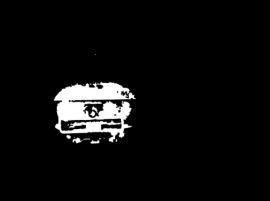
\includegraphics[width=0.5\linewidth]{figuras/sustraccion_mascara.png}
  \caption{Sustracción de Imágenes: Máscara de nuevos objetos}
  \label{fig:sustraccion_mascara}
\end{figure}

\begin{figure}[H]
  \centering
  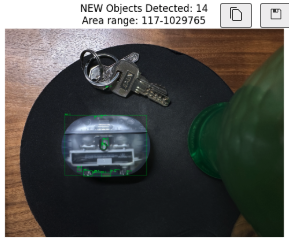
\includegraphics[width=0.5\linewidth]{figuras/sustraccion_objetos.png}
  \caption{Sustracción de Imágenes: Objetos detectados}
  \label{fig:sustraccion_objetos}
\end{figure}

Se observa que como resultado de la sustracción se produce una máscara de objetos nuevos (Figura \ref{fig:sustraccion_mascara}) que es predominantemente negra. Las áreas que han cambiado (donde está la caja de los audífonos) se muestran en blanco, creando un mapa que aísla el objeto en movimiento del fondo estático. La imagen final (figura \ref{fig:sustraccion_objetos}) superpone esta detección, mostrando el audífono enmarcado y los detalles de los objetos detectados. Este proceso es efectivo y de bajo costo para sistemas de monitoreo en tiempo real.

\newpage

\section{Conclusiones}

El proyecto permitió aplicar y analizar diversas transformaciones fotométricas pixel a pixel, demostrando su utilidad en la mejora visual de imágenes y en la preparación de datos para modelos de inteligencia artificial. Las técnicas implementadas no solo mejoran el contraste y la visibilidad de detalles, sino que también permiten generar variaciones útiles para entrenar redes neuronales. La integración de análisis visual y de histogramas fortaleció la comprensión del impacto de cada transformación. Se concluye que el procesamiento de imágenes es una herramienta clave en sistemas de visión computacional aplicados a medicina, seguridad, astronomía y clasificación automática. 

\newpage

% ==============================
% REFERENCIAS - SOLO UNA VEZ
% ==============================
\begin{thebibliography}{99}

\bibitem{anitha2018}
P. S. Anitha, P. Lakshmi Priya. (2018). A Survey on Image Enhancement Techniques. International Journal of Scientific Research in Computer Science and Engineering.

\bibitem{gonzalez2018}
R. C. Gonzalez and R. E. Woods, \textit{Digital Image Processing}, 4th ed., Pearson, 2018.

\bibitem{opencv}
OpenCV-Python Tutorials, OpenCV Official Documentation, 2023. Disponible en: \url{https://docs.opencv.org/4.x/}

%% Debemos usar Wikipedia como referencia?
\bibitem{wikipedia2023}
Wikipedia. (2023). Gamma correction. Disponible en: \url{https://en.wikipedia.org/wiki/Gamma_correction}

\end{thebibliography}

% ==============================
% NOTAS PARA RESOLVER PROBLEMAS DE COMPILACIÓN
% ==============================
% Si experimentas timeout en la compilación:
% 
% 1. IMÁGENES: Optimiza las imágenes antes de subirlas
%    - Reduce la resolución a 150-300 DPI máximo
%    - Usa formatos comprimidos: JPG para fotos (calidad 80-90%)
%    - Redimensiona a tamaño real de uso (no más de 1500px de ancho)
%    - Herramientas: ImageMagick, TinyPNG, o Squoosh.app
%
% 2. COMPILACIÓN RÁPIDA: Para pruebas, usa modo draft
%    - Cambia \usepackage{graphicx} por \usepackage[draft]{graphicx}
%    - Esto muestra solo los marcos de las imágenes
%
% 3. SI PERSISTE EL PROBLEMA:
%    - Compila localmente con TeXLive o MiKTeX
%    - Usa un plan de pago en Overleaf para más tiempo de compilación
%    - Divide el documento en archivos separados con \input{}

\end{document}